\title{\textbf{Automatic Projector Tilt Compensation System}}
\author{Ganesh Ajjanagadde \quad James Thomas \quad Shantanu Jain}
\date{\today}
\documentclass{article}

\usepackage{graphicx} % for including images
\usepackage{float} % for floating figures, i.e can place/modify images in fancy ways

%Please place images in img/ subdir of proj_proposal for clean directory structure

\begin{document}
\maketitle

%\begin{abstract}
%Our goal is to design a system that corrects the input to a projector if it is tilted so that its output appears unskewed.
%We will be projecting the display of a PC, and will connect the computer's VGA output to the FPGA board, and the FPGA board's VGA output to the projector.
%We will mount an accelerometer on the projector and measure its signals to determine the projector's tilt angles on two axes.
%We will run algorithms on the FPGA that correct the VGA input based on the tilt angles and produce the results at the VGA output for the projector to display.
%Finally, we will design digital logic that produces a voice specifying the new tilt angles whenever they are changed.
%The project was motivated by the increasing prevalance of portable projectors that benefit from fast automated setup.
%\end{abstract}

\section{Introduction}
%TODO: Fill out introduction/motivation (Ganesh)

\section{Implementation}

\subsection{Block Diagram}
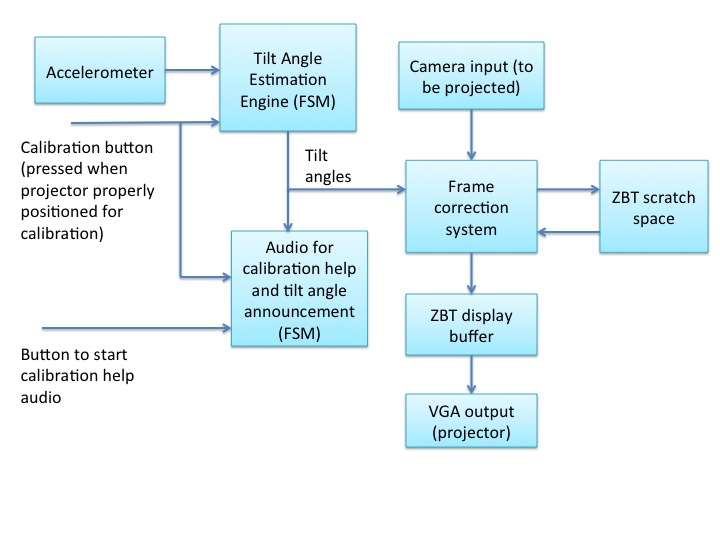
\includegraphics{img/block_diag}

\subsection{Modules}
\begin{description}
	\item{Accelerometer}
	\begin{itemize}
		\item Includes logic to convert signals from the accelerometer (whether in analog or SPI digital format) to normalized digital values that can be fed to the tilt angle estimation engine
	\end{itemize}
	\item{Tilt angle estimation engine}
	\begin{itemize}
		\item When calibration button is pressed, updates state to set the current values from the accelerometer as the reference values for an untitled projector
		\item By comparing the values from the accelerometer to the stored reference values, produces estimates of the angles of tilt in the two axes of interest
	\end{itemize}
	\item{Audio}
	\begin{itemize}
		\item When the calibration help button is pressed, goes into state in which it periodically plays a recording instructing the user to adjust the projector so that its output looks unskewed and then hit the calibration button
		\item When the calibration button is pressed, exits the help state if it is in it
    \item When a change in the current angles of projector tilt is detected, plays recordings that specify the angles
		\item Audio samples are stored on compact flash
	\end{itemize}
  \item{Frame correction system}
	\begin{itemize}
		\item Based on the current angles of projector tilt, adjusts an incoming frame from the camera using a linear transformation (implemented with a matrix multiplication) so that when it is projected it appears unskewed
		\item Uses the ZBT scratch space to store each frame from the camera (reading pixels from the stored frame for the matrix multiplication) and possibly the results of intermediate computations
    \item Stores the output frame from the linear transformation in a display buffer (also ZBT)
    \item An auxiliary module will feed the pixels in the display buffer to the VGA output at the appropriate clock edges
	\end{itemize}
\end{description}



\section{Timeline}
%TODO: Add a week by week timeline (Shawn), Gantt chart if it is not too hard
There is five weeks time in which to complete the project. In these five weeks, we envision four major stages to the project: 
\begin{enumerate}
	\item Initial attempt at implementing each block \hfill \\
		Time: 2 weeks \hfill \\
		In this stage, each team member will create an initial implementation of modules he is responsible for. He is expected to have his modules working as a standalone component. Each module will include simple test benches in order to facilitate this goal. 
	\item Module Integration; System Building \hfill \\
		Time: 2 weeks \hfill \\
		This stage will connect the individual modules from stage 1 together to form the initial system. This is expected to be the most hands-on and collaborative stage, as mistakes will often have a domino effect on the system. In the worst case, we may have to modify parts of our system design or change the behavior of some modules in order to compensate; in lesser situations, bugs may be uncovered and fixed. This is expected to be the lengthiest stage. 
	\item Intensive debugging \hfill \\
		Time: 1 week \hfill \\
		After the system has been put together and functions minimally, the team will focus on debugging. The goal of debugging is to make the system robust. Testing will include the common usage scenarios as well as edge cases, and a limited set of malicious inputs. 
	\item Stretch Goals \hfill \\ 
		Time: As available \hfill \\
		Once the system satisfies the test coverage plan, the team will focus on adding additional features to the system, as constrained by time. These possible additional features are described below.

\end{enumerate}

\section{Individual Responsibility}
\begin{description}
	\item{Ganesh}
	\begin{itemize}
		\item Algorithm - Identifying the appropriate algorithm, considering factors of complexity, hardware constraints, and implementability. 
		\item Transform Module - Implementing the algorithm, with input parameters
	\end{itemize}
	\item{James}
	\begin{itemize}
		\item Accelerometer - Identifying the appropriate type and model, interfacing with the labkit.
		\item Calibration module - Entering calibration mode, collecting data, making it available as necessary. 
	\end{itemize}
	\item{Shantanu}
	\begin{itemize}
		\item Audio output - Identifying necessary audio outputs, triggers for audio. Recording audio, transforming it into the appropriate format. 
		\item Audio module - loading audio onto the labkit, standardizing trigger parameters. 
		\item Test Setup - attaching accelerometer to projector, wiring to labkit. 
	\end{itemize}
\end{description}

\section{Stretch Goals}
	\begin{itemize}
		\item Camera-based adjustment \hfill \\
			The camera-based adjustment would augment the accelerometer by displaying a test pattern output to the projector and using an edge detection/corner detection algorithm to determine the skew caused by the projector's tilt. It would be able to correct the projector image in a wider variety of scenarios, including variable distance to the screen. This is difficult as it is complex and time consuming to interface the camera with the labkit and implement these additional algorithms. 
		\item External display of transformed image\hfill \\
			View the transformed image on a non-distorted screen, such as a PC LCD monitor. 
	\end{itemize}
\end{document}
